\documentclass{beamer}
\usepackage{amsmath}
\usepackage[utf8]{inputenc}
\usepackage{xmpmulti}

\mode<presentation>{
\definecolor{cured}{rgb}{.8,0,.2}
\usecolortheme[named=cured]{structure}
\usetheme{split}
}

\newcommand{\taco}{\raisebox{-.1ex}{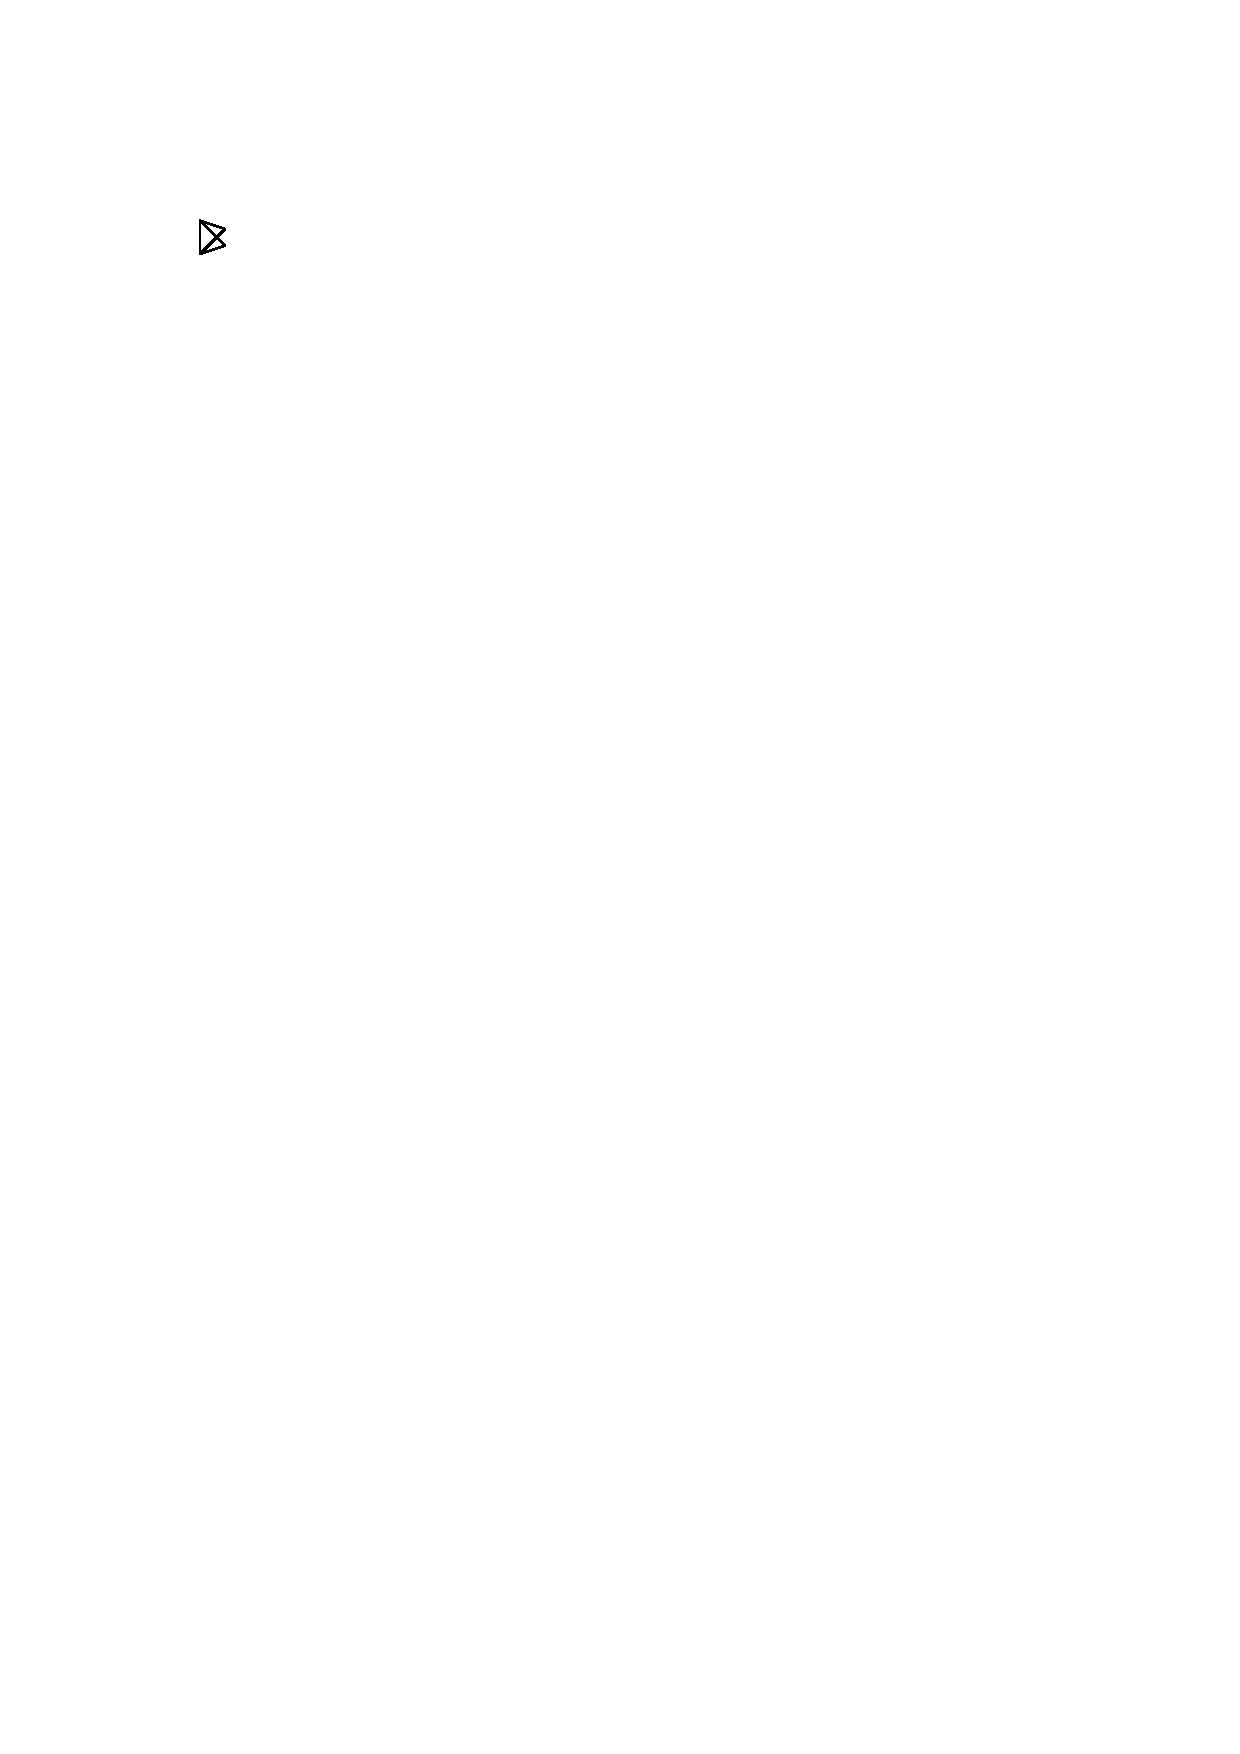
\includegraphics[height=2.0ex]{figs/triangles-edge-1}}}
\newcommand{\mariposa}{\raisebox{-.1ex}{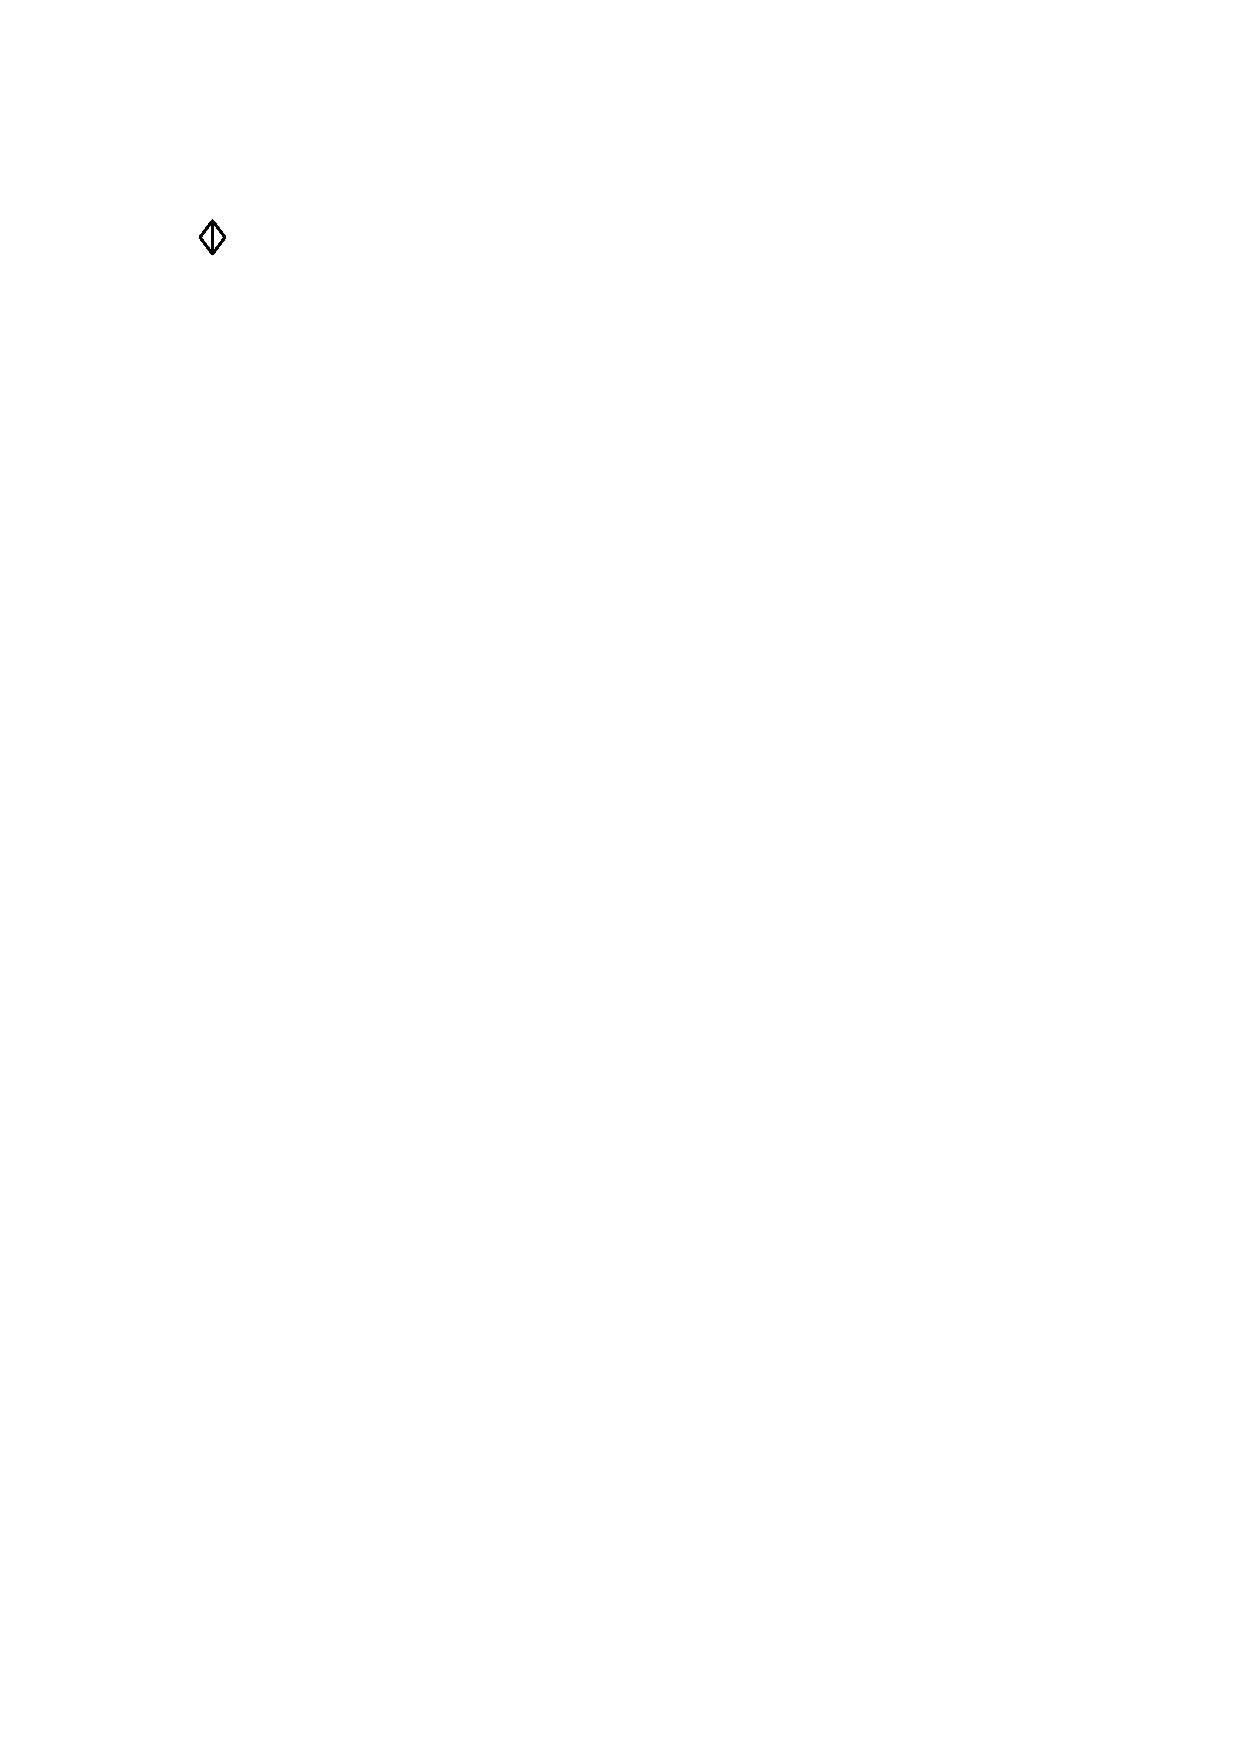
\includegraphics[height=2.0ex]{figs/triangles-edge-2}}}


\newcommand{\bat}{\raisebox{-.1ex}{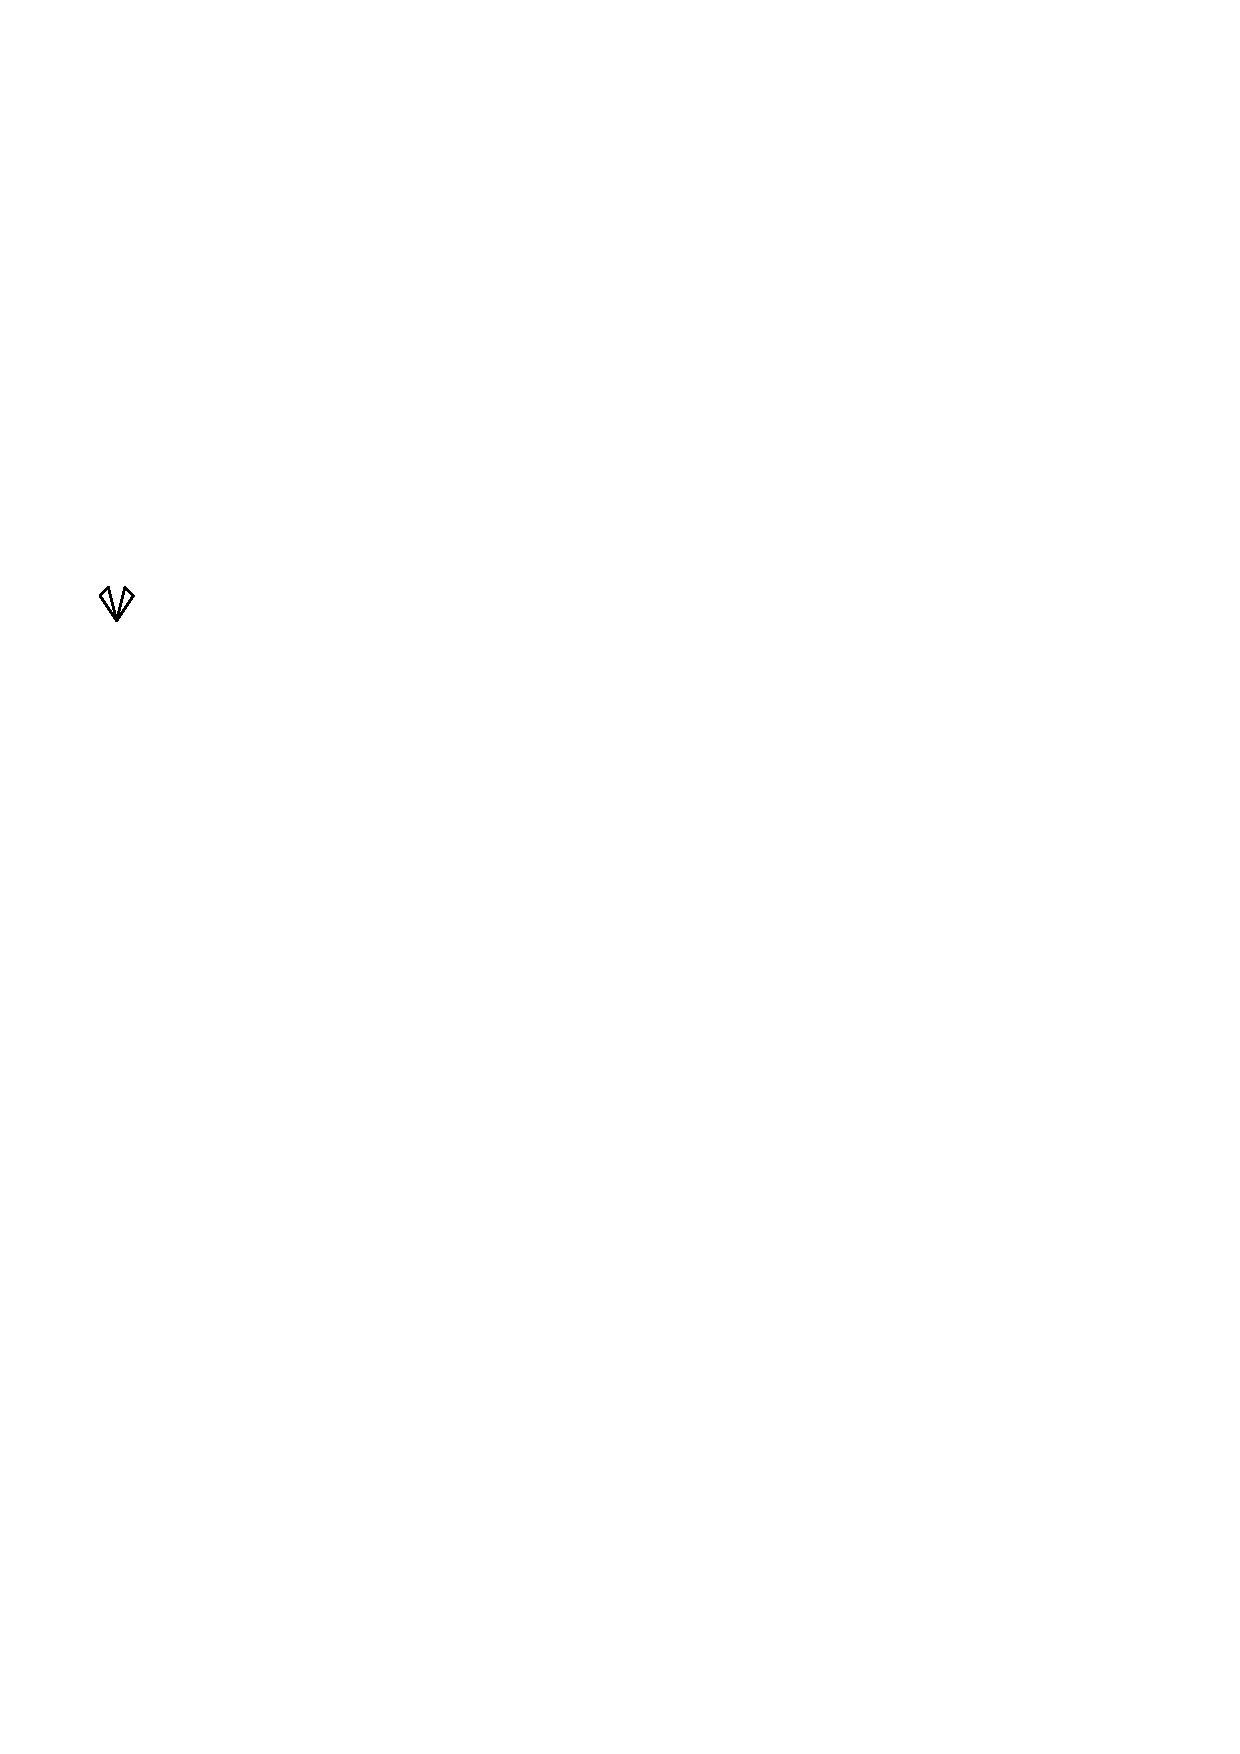
\includegraphics[height=2.0ex]{figs/triangles-vertex-1}}}
\newcommand{\nested}{\raisebox{-.1ex}{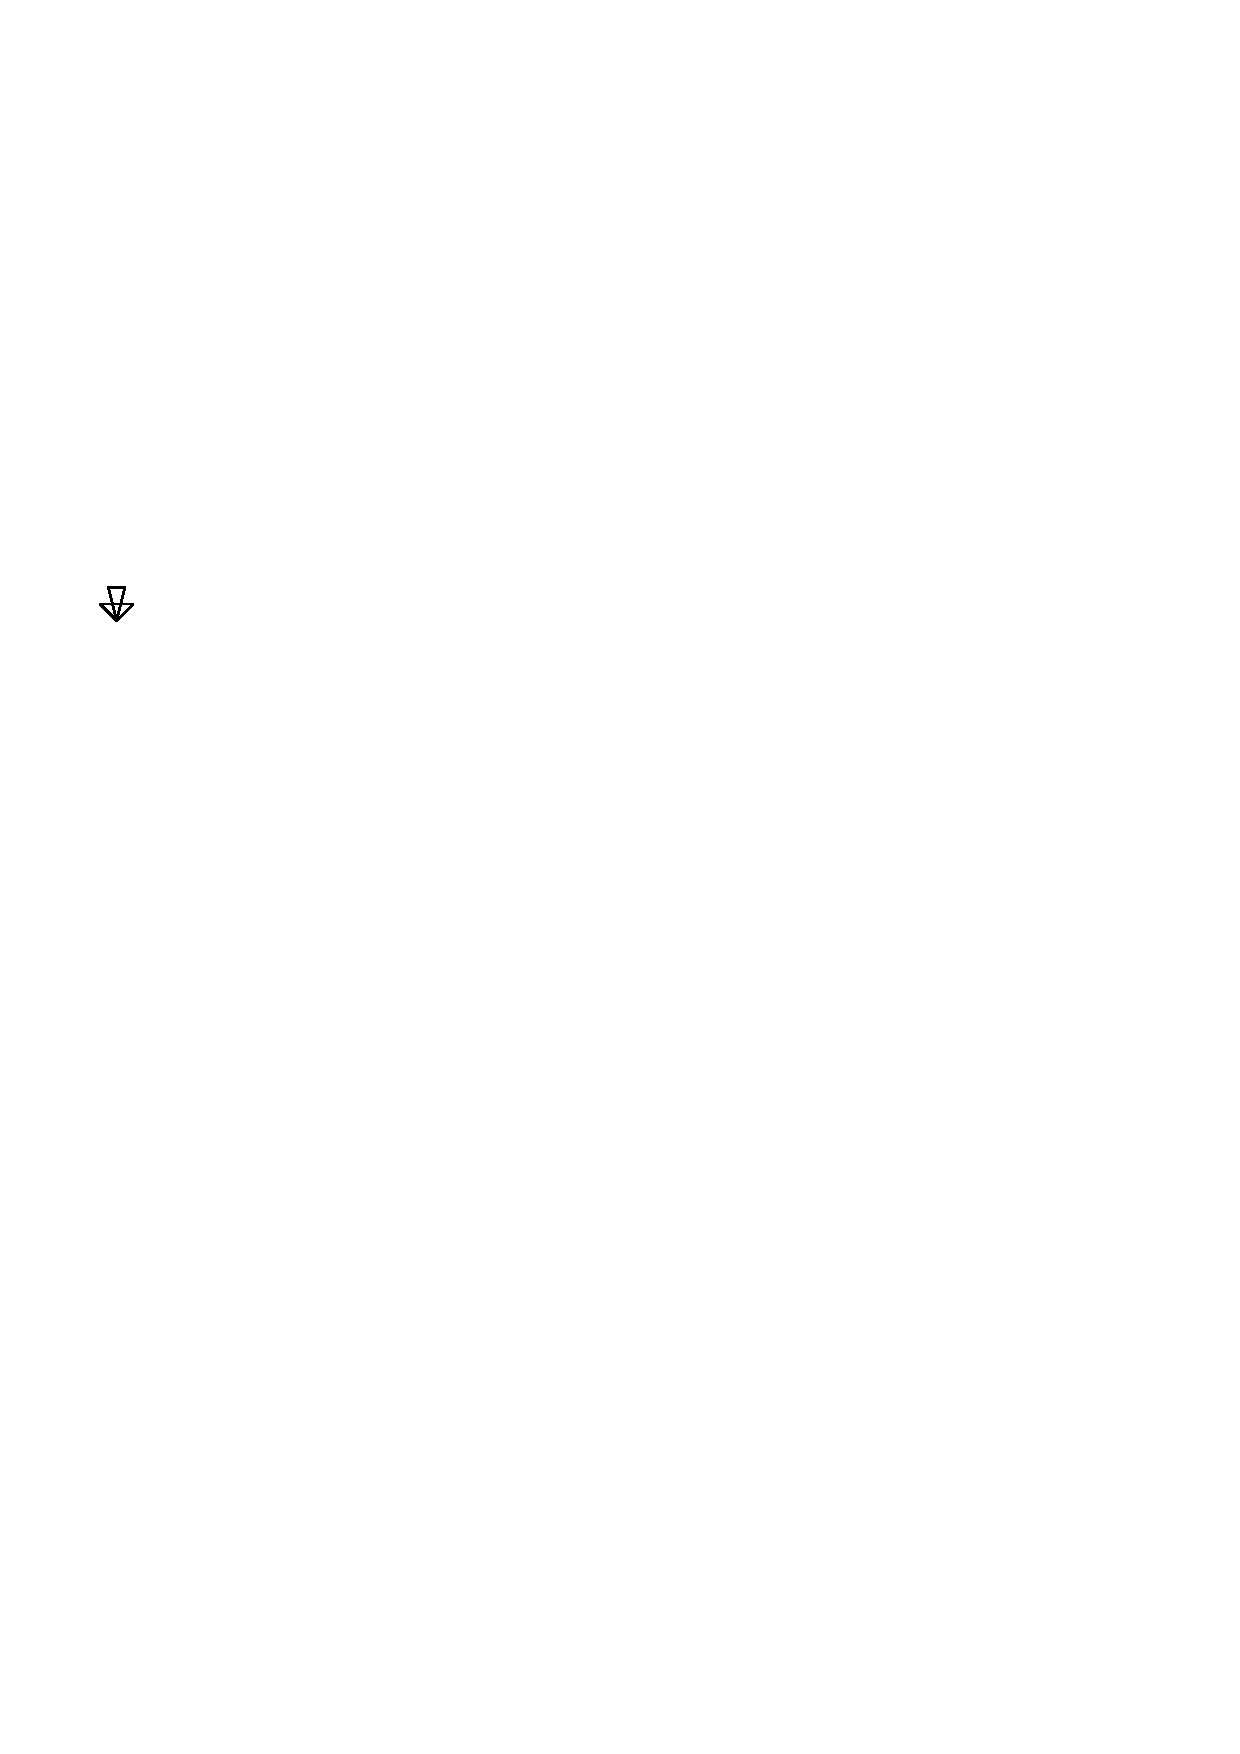
\includegraphics[height=2.0ex]{figs/triangles-vertex-2}}}
\newcommand{\crossing}{\raisebox{-.1ex}{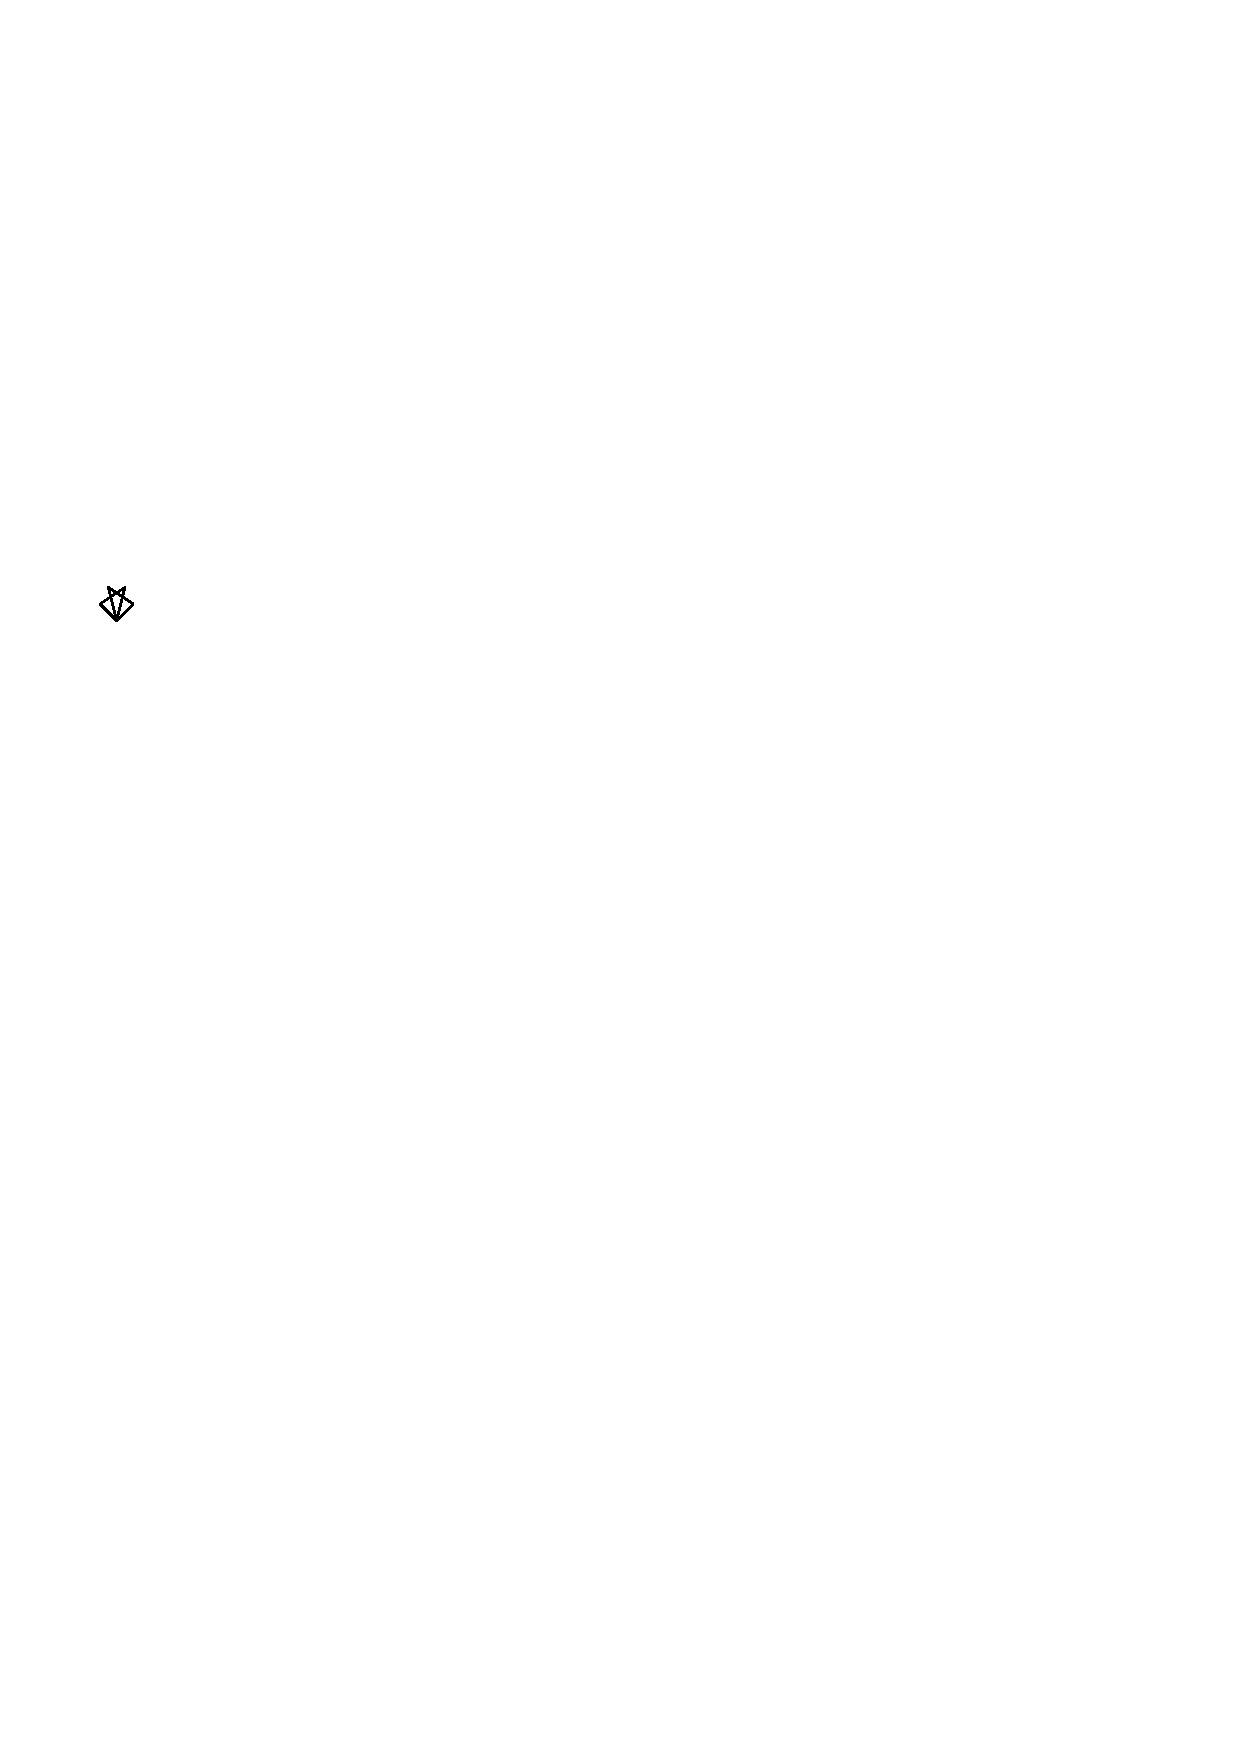
\includegraphics[height=2.0ex]{figs/triangles-vertex-3}}}

\newcommand{\ears}{\raisebox{-.1ex}{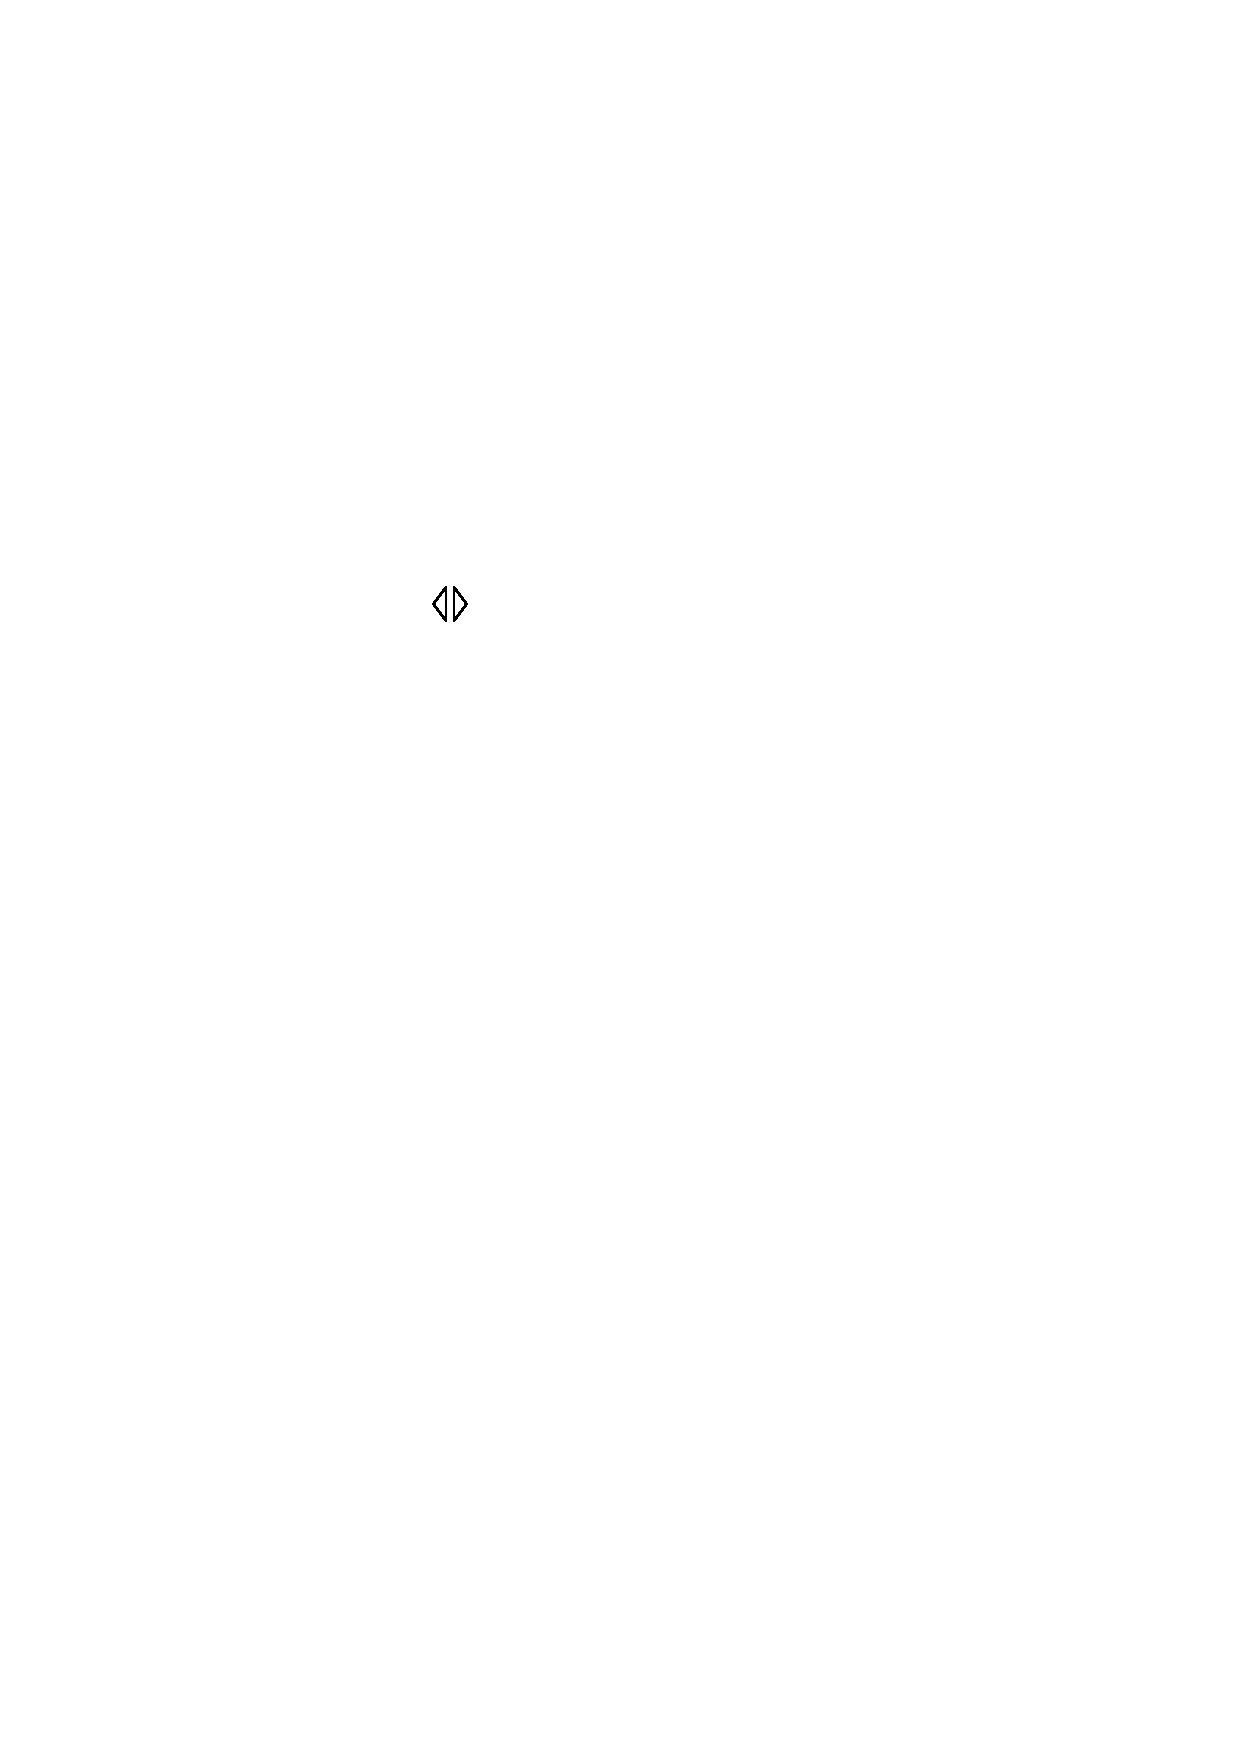
\includegraphics[height=2.0ex]{figs/triangles-disjoint-1}}}
\newcommand{\swords}{\raisebox{-.1ex}{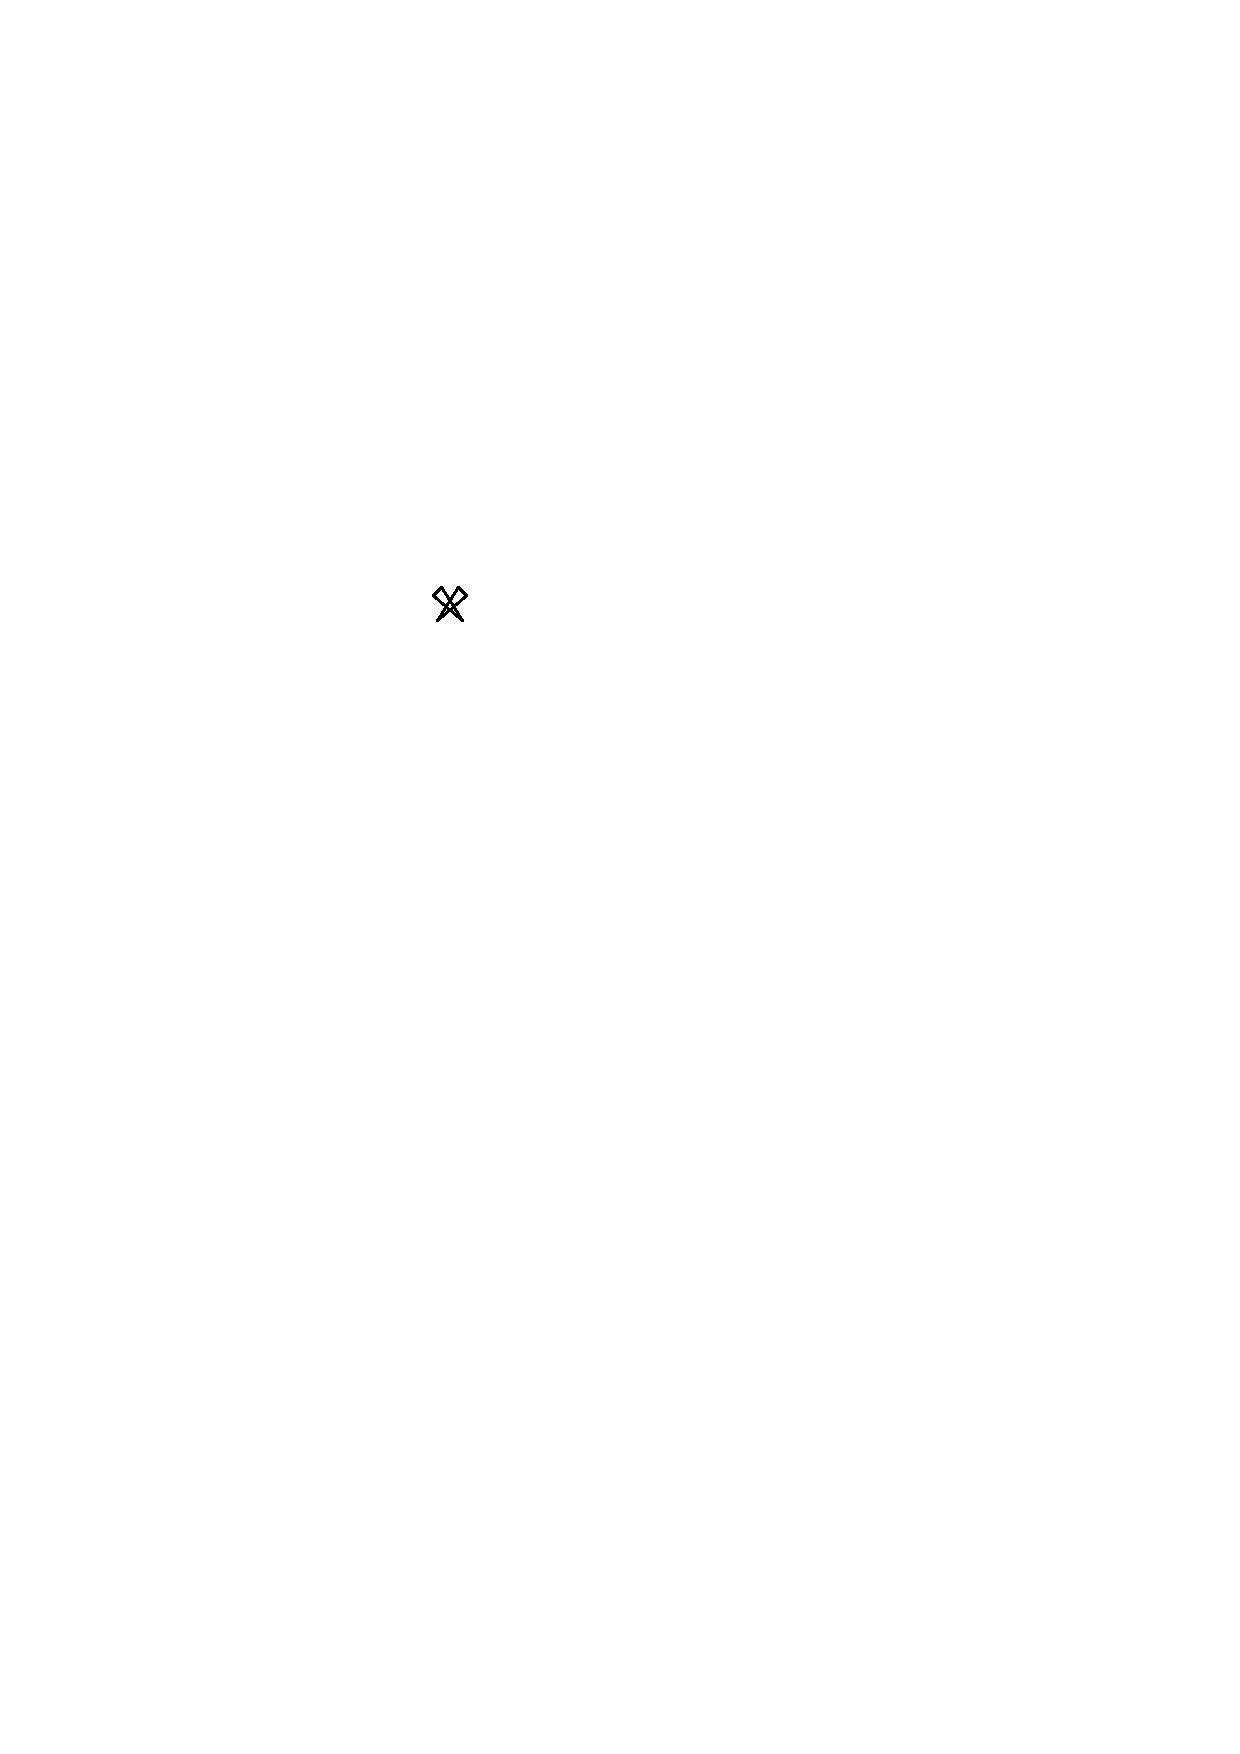
\includegraphics[height=2.0ex]{figs/triangles-disjoint-2}}}
\newcommand{\david}{\raisebox{-.1ex}{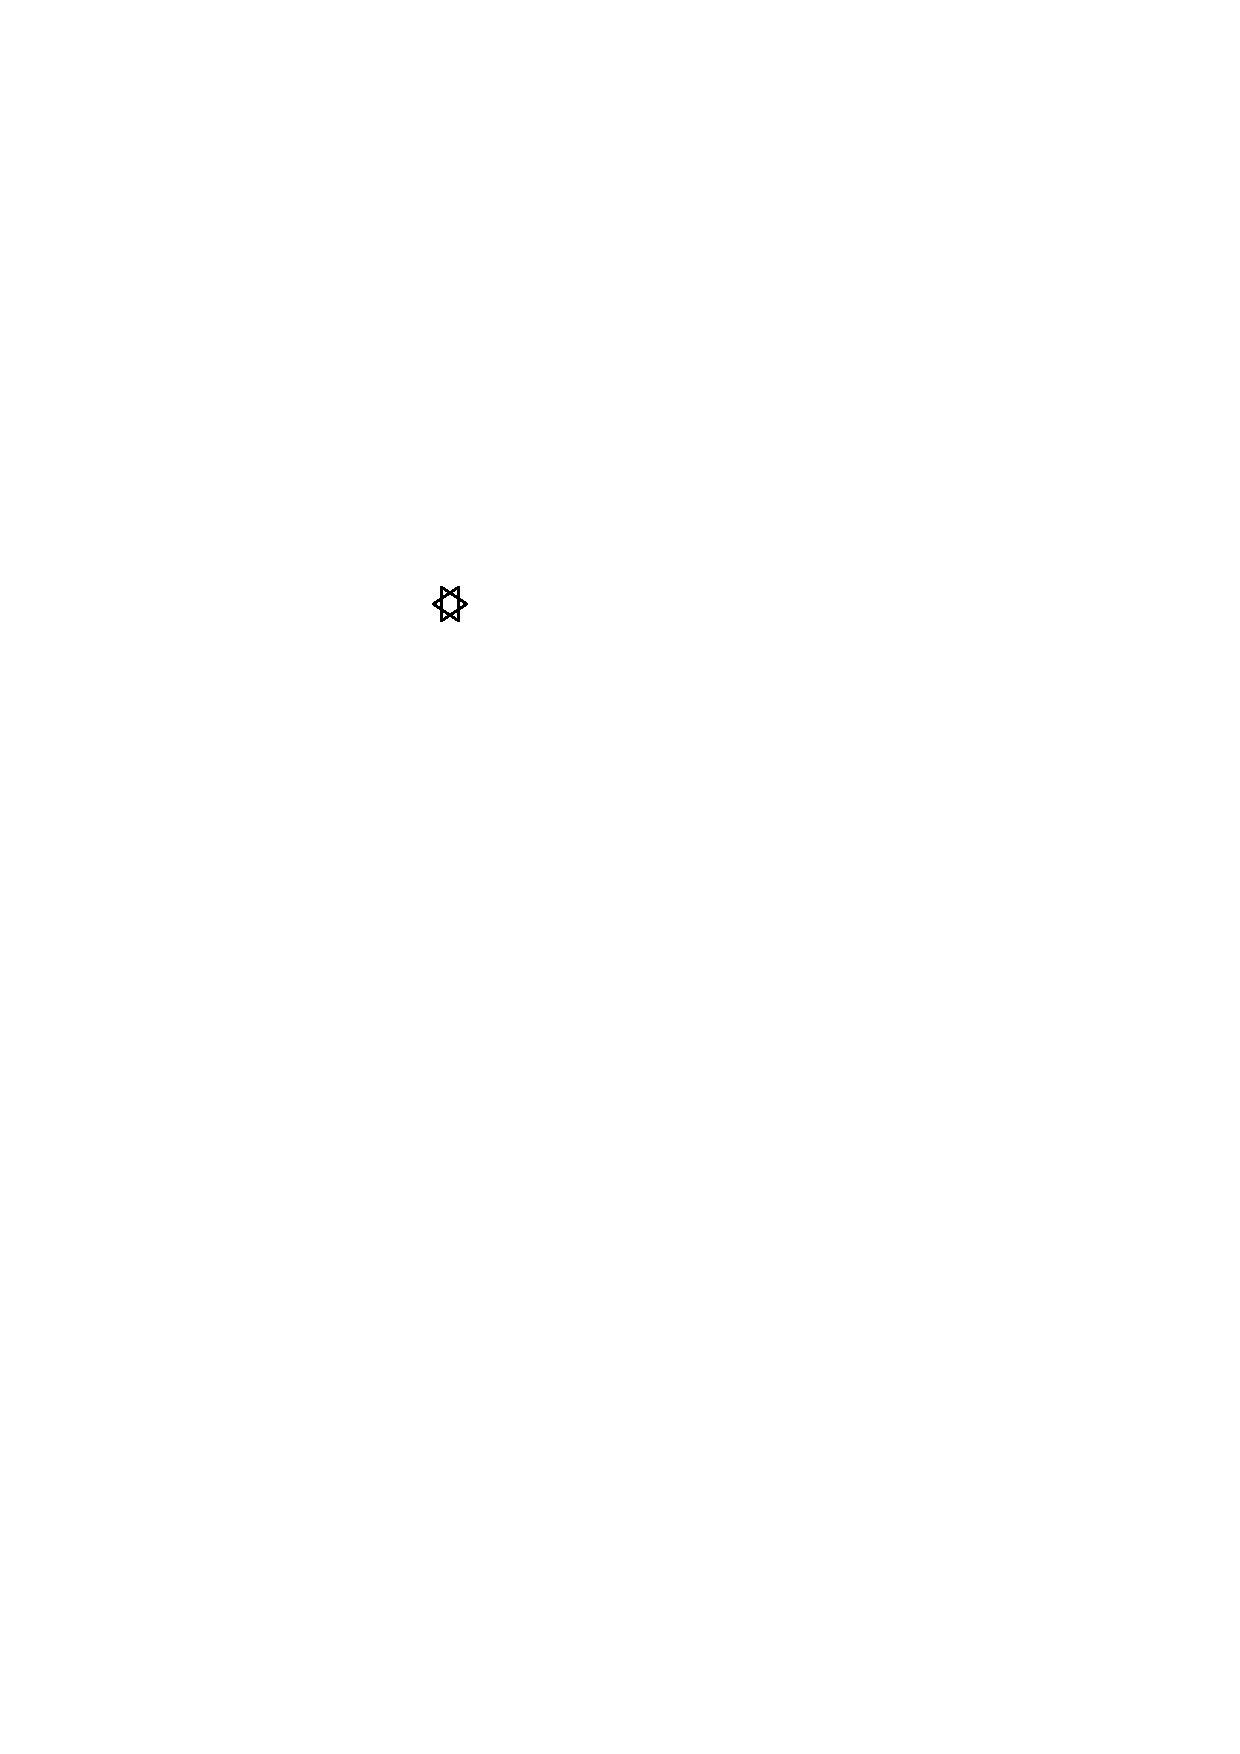
\includegraphics[height=2.0ex]{figs/triangles-disjoint-3}}}


\newcommand{\mi}[1]{\multiinclude[<+>][start=1,format=pdf]{#1}}

\DeclareMathOperator{\ex}{ex}

 
\usepackage{amsthm}

\newcommand{\centeripe}[1]{\begin{center}\Ipe{#1}\end{center}}
\newcommand{\comment}[1]{}

\newcommand{\centerpsfig}[1]{\centerline{\psfig{#1}}}

\newcommand{\seclabel}[1]{\label{sec:#1}}
\newcommand{\Secref}[1]{Section~\ref{sec:#1}}
\newcommand{\secref}[1]{\mbox{Section~\ref{sec:#1}}}

\newcommand{\alglabel}[1]{\label{alg:#1}}
\newcommand{\Algref}[1]{Algorithm~\ref{alg:#1}}
\newcommand{\algref}[1]{\mbox{Algorithm~\ref{alg:#1}}}

\newcommand{\applabel}[1]{\label{app:#1}}
\newcommand{\Appref}[1]{Appendix~\ref{app:#1}}
\newcommand{\appref}[1]{\mbox{Appendix~\ref{app:#1}}}

\newcommand{\tablabel}[1]{\label{tab:#1}}
\newcommand{\Tabref}[1]{Table~\ref{tab:#1}}
\newcommand{\tabref}[1]{Table~\ref{tab:#1}}

\newcommand{\figlabel}[1]{\label{fig:#1}}
\newcommand{\Figref}[1]{Figure~\ref{fig:#1}}
\newcommand{\figref}[1]{\mbox{Figure~\ref{fig:#1}}}

\newcommand{\eqlabel}[1]{\label{eq:#1}}
%\newcommand{\eqref}[1]{(\ref{eq:#1})}
\newcommand{\Eqref}[1]{Equation~(\ref{eq:#1})}

\newtheorem{thm}{Theorem}{\bfseries}{\itshape}
\newcommand{\thmlabel}[1]{\label{thm:#1}}
\newcommand{\thmref}[1]{Theorem~\ref{thm:#1}}

\newtheorem{lem}{Lemma}{\bfseries}{\itshape}
\newcommand{\lemlabel}[1]{\label{lem:#1}}
\newcommand{\lemref}[1]{Lemma~\ref{lem:#1}}

\newtheorem{cor}{Corollary}{\bfseries}{\itshape}
\newcommand{\corlabel}[1]{\label{cor:#1}}
\newcommand{\corref}[1]{Corollary~\ref{cor:#1}}

\newtheorem{obs}{Observation}{\bfseries}{\itshape}
\newcommand{\obslabel}[1]{\label{obs:#1}}
\newcommand{\obsref}[1]{Observation~\ref{obs:#1}}

\newtheorem{cond}{Condition}{\bfseries}{\itshape}

\newtheorem{clm}{Claim}{\bfseries}{\itshape}
\newcommand{\clmlabel}[1]{\label{clm:#1}}
\newcommand{\clmref}[1]{Claim~\ref{clm:#1}}


\newtheorem{dfn}{Definition}{\bfseries}{\rm}

\newtheorem{assumption}{Assumption}{\bfseries}{\rm}
\newenvironment{ass}{\begin{assumption}\rm}{\end{assumption}}
\newcommand{\asslabel}[1]{\label{ass:#1}}
\newcommand{\assref}[1]{Assumption~\ref{ass:#1}}

\newcommand{\proclabel}[1]{\label{alg:#1}}
\newcommand{\procref}[1]{Procedure~\ref{alg:#1}}

\newtheorem{rem}{Remark}
\newtheorem{op}{Open Problem}

\newcommand{\etal}{\emph{et al}}

%\newcommand{\keywords}[1]{\noindent\textbf{Keywords:} #1}
\newcommand{\voronoi}{Vorono\u\i}
\newcommand{\ceil}[1]{\left\lceil #1 \right\rceil}
\newcommand{\floor}[1]{\left\lfloor #1 \right\rfloor}
\newcommand{\R}{\mathbb{R}}
\newcommand{\N}{\mathbb{N}}
\newcommand{\Z}{\mathbb{Z}}
\newcommand{\Sp}{\mathbb{S}}
\newcommand{\E}{\mathrm{E}}

\usepackage{marvosym}

\newcommand{\notice}[1]
{
   {\Lightning}
   \marginpar{
      \begin{flushleft}\raggedright
        \hspace{-1.5mm}\Lightning{\small #1}
      \end{flushleft}
   }
}



\title{Turán-Type Theorems for Triangles in Convex Point Sets}
\author{Pat Morin}
\date{January 29, 2016}

\begin{document}

\begin{frame}
  \titlepage
\end{frame}

\begin{frame}
  \frametitle{Maximum Triangles Problem}
  \framesubtitle{Erd\H{o}s and Purdy (1971)}

  \begin{itemize}
      \item What is the largest number of
        maximum area triangles determined by a set of $n$ points?
      \centerline{\mi{slidefigs/erdos-regular}}%
      \item<2->At least $n$
  \end{itemize}
\end{frame}

\begin{frame}
  \frametitle{Maximum Triangles Problem}
  \framesubtitle{Bra\ss, Rote, Swanepoel (2001)}

  \textbf{Theorem:} Any set of $n$ points determines at most $n$ maximum-area triangles
  \begin{itemize}[<+->]
      \item WLOG we can assume points are in convex position
      \item How can a pair of maximum area triangles interleave?
      \begin{itemize}
         \item Like this: \taco, \david, \crossing, \mariposa
         \item Not like this: \ears, \swords, \nested, \bat
      \end{itemize}
      \item What is the maximum number of triangles we can draw on a convex
         $n$-gon before we
         get a pair that like  \ears, \swords, \nested, or \bat?
  \end{itemize}
\end{frame}

\begin{frame}
  \frametitle{Maximum Triangles Problem}
  \framesubtitle{Bra\ss, Rote, Swanepoel (2001)}

  Let $\ex(n,X)$ denote the maximum number of triangles we can draw on a convex $n$-gon before we get a configuration from $X$.

  \textbf{Theorem (BRS2001):} $\ex(n,\{\ears,\swords,\nested,\bat\})\le n$.

  \begin{itemize}[<+->]
     \item Number polygon vertices $0,\ldots,n-1$
     \item Represent each triangle as a triple: $(a,b,c)$, with $0\le a<b<c<n$.
     \item Order triangles according to 
         \[ (a,b,c)\preceq (d,e,f) \Leftrightarrow a\le d, b\le e, c\le f \] 
     \item Key insight: Any pair of triangles (\taco, \david, \crossing, \mariposa) is comparable! 
     \item $\Delta_1<\Delta_2<\cdots<\Delta_k \Rightarrow k \le 3n$
     \item Count a bit more carefully to get $k\le n$ \hfill{QED}
  \end{itemize}
\end{frame} 

\begin{frame}
  \frametitle{Turán-Type Theorems for Triangles in Convex Point Sets}
  \framesubtitle{256 Problems}

   \begin{itemize}[<+->]
      \item $\ex(n,X)$ is the maximum number of triangles we can draw on 
         a convex $n$-gon before we get a configuration from $X$
 
      \item 256 problems: Determine $\ex(n,X)$ for every $X\subseteq\{\taco,\david,\crossing,\mariposa,\ears,\swords,\nested,\bat\}$
      \item Bra\ss\ (2004): \\
        \[ \begin{array}{rrr}
           \ex(n,\{\ears\})=\Theta(n^3) & \ex(n,\{\swords\})=\Theta(n^2) & \ex(n,\{\david\})=\Theta(n^2) \\
           \ex(n,\{\bat\})=\Theta(n^3) & \ex(n,\{\nested\})=\Theta(n^2) & \ex(n,\{\crossing\})=\Theta(n^2) \\
           \ex(n,\{\mariposa\})=\Theta(n^3) & \ex(n,\{\taco\})=\Theta(n^2) 
           \end{array}
        \]
        \[\begin{array}{r}
           \ex(n,\{\bat,\nested\})=\Theta(n^2) \\ \ex(n,\{\crossing,\nested\})=\Theta(n^2) \\ \ex(n,\{\bat,\crossing\})=\Theta(n^2) \\
        \end{array}\]
   \end{itemize}
\end{frame}

\begin{frame}
  \frametitle{Proof that $\ex(n,\{\crossing\})=O(n^2)$}

  \centerline{\mi{slidefigs/crossing}}
\end{frame} 


\begin{frame}
  \frametitle{Proof that $\ex(n,\{\swords\})=O(n^2)$}

  \centerline{\mi{slidefigs/swords}}
\end{frame} 


\begin{frame}
  \frametitle{Proof that $\mariposa$ doesn't matter}

   \textbf{Theorem:} Any set of triangles of size $N$ contains a subset
    of size at least $N/8$ that has no \mariposa\ pair
  \begin{itemize}[<+->]
   \item Randomly direct each pair $u,v$ of vertices ($\overrightarrow{uv}$ or $\overleftarrow{uv}$)
   \item Discard all triangles that use $uv$ and are on the right of $uv$
   \item Resulting set has expected size $N/8$ and no $\mariposa$ pairs
  \end{itemize} 
\end{frame} 


\begin{frame}
  \frametitle{The Top-Bottom View}

   Let $\ex'(n,X)$ be the just like $\ex(n,X)$ but we only count triangles
   with one vertex in the bottom half and two in the top half.

   \centerline{top-bottom}

   \textbf{Theorem:} Any set of triangles of size $N$ contains a subset
    of size at least $N/8$ that has no \mariposa\ pair
  \begin{itemize}[<+->]
   \item Randomly direct each pair $u,v$ of vertices ($\overrightarrow{uv}$ or $\overleftarrow{uv}$)
   \item Discard all triangles that use $uv$ and are on the right of $uv$
   \item Resulting set has expected size $N/8$ and no $\mariposa$ pairs
  \end{itemize} 
\end{frame} 


\end{document}

